\chapter{Реализация}

% В этой главе описывается, что и как было запрограммировано, отлажено, 
% протестировано, и что в результате получилось. Большинство работ должны 
% содержать приведенные ниже разделы. Но нужно учитывать, что точный состав 
% этой главы, как и других глав, зависит от специфики работы.

% Фрагменты программного кода в тексте необходимо выделять при помощи команды 
% \verb|\verb|. Многострочные листинги должны оформляться при помощи пакета 
% \verb|listings|. Пример:

% \begin{lstlisting}
% # let s x y z = x z (y z);;
% val s : ('a -> 'b -> 'c) -> ('a -> 'b) -> 'a -> 'c = <fun>
% # let k x y = x;;
% val k : 'a -> 'b -> 'a = <fun>
% # let i = s k k;;
% val i : '_a -> '_a = <fun>
% \end{lstlisting}

% Листинг \ref{lst:float-example} иллюстрирует использование выносных листингов.
% Листинг \ref{lst:HelloWorld.scala} показывает пример включения внешнего файла 
% в качестве листинга, в данном случае --- выносного.

% \begin{lstlisting}[
%   float=tb,frame=lines,label=lst:float-example,caption=Выносной листинг
% ]
% List myList = new List();
% Element myElement = new Element();
% myList.Append(myElement);
% \end{lstlisting}

% \lstinputlisting[
%   label=lst:HelloWorld.scala,
%   float=tb,frame=lines,
%   caption=Листинг из файла \texttt{HelloWorld.scala}
% ]{listings/HelloWorld.scala}


\section{Состав и структура реализованного программного обеспечения}

Реализованно серверное приложение, отвечающие на запросы по HTTP.

\subsection{Структура приложения}
Приложение состоит из 5 микросервисов:
\begin{itemize}
  \item Gateway API
  \item Auth Service
  \item Uzi Service
  \item Med Service
  \item Ml Service
\end{itemize}

Каждый микросервис написанный на golang содержит:
\begin{itemize}
  \item go.mod и go.sum файлы, описывающие библиотекчные зависимости для приложения
  \item sql файлы миграций. Сами миграции осуществлялись за счет Goose
  \item md файлы с описанием технических требований к предоставляемому API сервиса
  \item proto файлы описывающие контракты для взаимодествия с внешними системами
  \item taskfile - аналог makefile, файл для локальной сборки и запуска микросервиса
  \item Dockerfile - файл для сборки docker образа микросервиса
  \item service.yml - файл содержащий конфигурацию сервиса
\end{itemize}


% Нужно охарактеризовать реализованное ПО: является ли оно настольной программной для Windows, 
% или веб-приложением в форме сайта/веб-сервиса, или модулем/подключаемой библиотекой, или 
% \dots. Также нужно перечислить, из чего оно состоит: какие исполняемые файлы и их назначение, 
% конфигурационные файлы, файлы баз данных, требования к программному и аппаратному окружению, и т.п.

% Если реализованное приложение достаточно обширно, этот раздел может быть
% разделен на несколько: один с общим описанием, и по одному на подсистемы самого
% верхнего уровня.



\section{Основные сценарии работы пользователя}
Основной сценарий работы ПО - отправка запросов на обработку узи изображений и полученние данных с
обработанных изображений. Для взаимодействием с сервисом предоставляется подробное swagger api.
\begin{figure}[H]%
	\begin{center}
		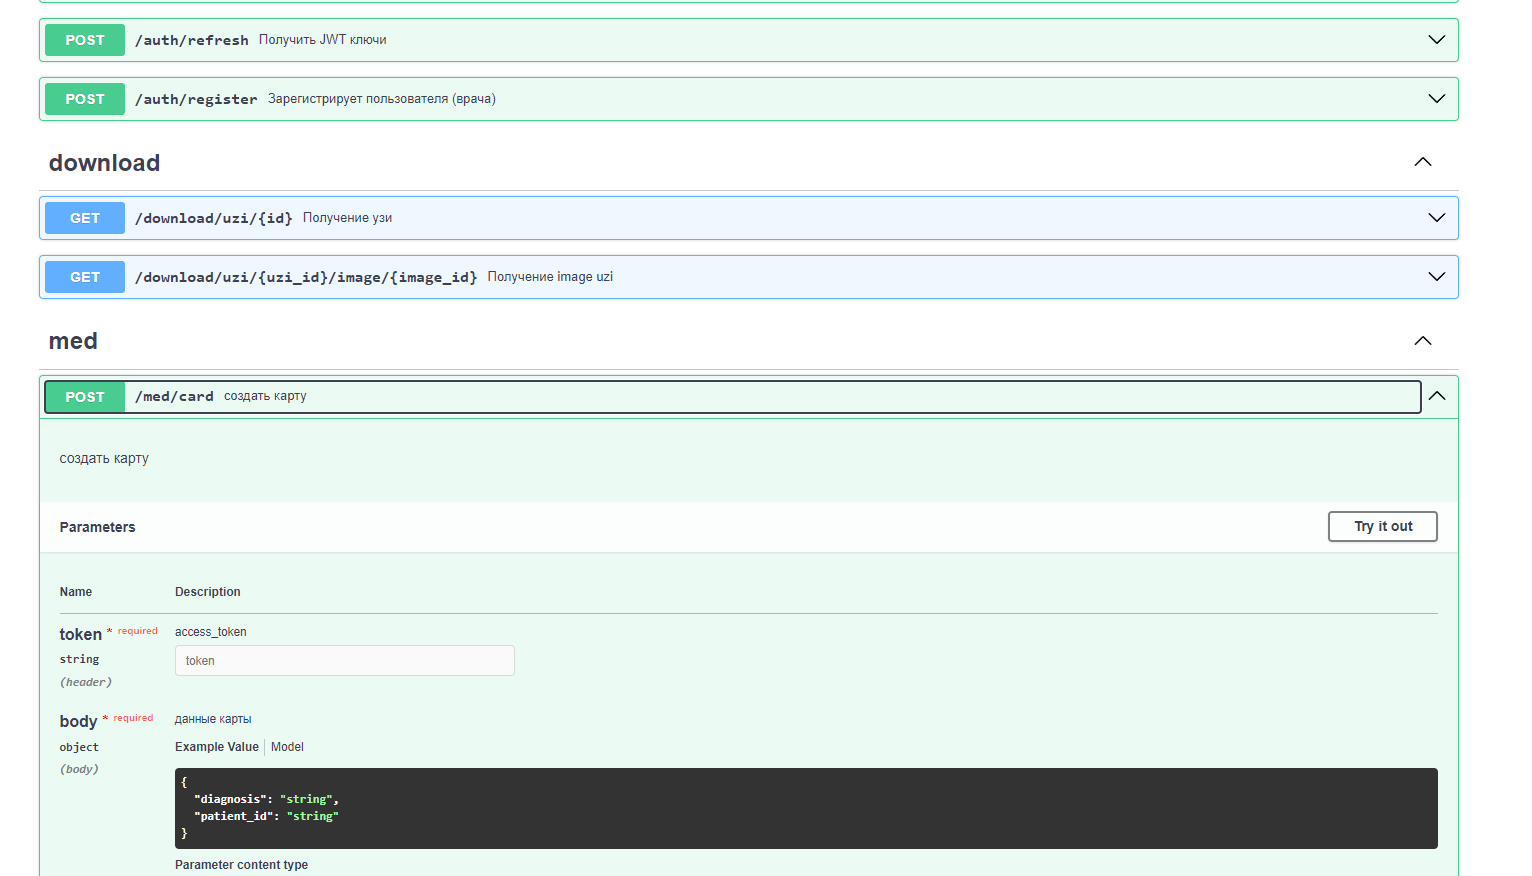
\includegraphics[width=.9\columnwidth]{./img/swagger.png}%
	\end{center}
	\caption{Спроектированная база данных Auth Service}%
	\label{pic:auth_model}%
\end{figure}

Подробнее в листинге.

% Нужно помнить, что пользователем может быть не только <<менеджер>> или <<человек в белом халате>>, 
% но и другой программист. Последнее относится, в первую очередь, к реализованным библиотекам. 
% Для <<обычных>> приложений нередко бывают пользователи нескольких категорий --- например, обычный 
% пользователь и администратор. Для каждой категории нужно описать, как выполняются основные функции, 
% предпочтительно, с помощью серии скрин-шотов. Однако считается плохим тоном вставлять длинную вереницу 
% из скрин-шотов: если их много, большую часть нужно выносить в приложение. Для \textit{этого} раздела 
% нормальной является плотность скрин-шотов из расчета: 1 страница скрин-шотов на 1-2 страницы текста.




\section{Выводы}
Таким образом, в рамках НИРа было реализовано 4 микросервиса серверного приложения, а также были проведены некоторые типы тестирования реализации. 
В будущем планируется развернуть систему на нескольких физическим машинах с использованием оркестратора контейнеризированных приложений 
kubernetus и повторно провести нагрузочное и интеграционное тестирование.

% Следует перечислить, какие практические результаты были получены, а именно: какое 
% программное или иное обеспечение было создано. В число результатов могут входить, 
% например, методики тестирования, тестовые примеры (для проверки корректности/оценки 
% характеристик тех или иных алгоритмов) и др. По каждому результату следует сделать вывод, 
% насколько он отличается от известных промышленных аналогов и исследовательских прототипов.



%%% Local Variables:
%%% TeX-engine: xetex
%%% eval: (setq-local TeX-master (concat "../" (seq-find (-cut string-match ".*-3-pz\.tex$" <>) (directory-files ".."))))
%%% End:
